%%%%%%%%%%%%%%%%%%%%%%%%%%%%%%%%%%%%%%%%%%%%%%%%%%%%
%    Canadian AI Latex Template    %
%%%%%%%%%%%%%%%%%%%%%%%%%%%%%%%%%%%%%%%%%%%%%%%%%%%%
\documentclass[10pt]{cai}

\begin{document}
% Editorial staff will replace the following values:
% 1. Conference Year
% 2. Issue number
% 3. Article DOI
\def\conferenceyear{2025}
\volumeheader{38}{0}%{00.000}
\begin{center}

\title{Development of a Reinforcement Learning Enabled Cattle Tracker Prototype}
\maketitle

\thispagestyle{empty}

% Add Authors and Affiliations in the camera ready
% for the double blind review, please leave this section as is 
\begin{tabular}{cc}
First Author\upstairs{\affilone,*}, Second Author\upstairs{\affilone}, Third Author\upstairs{\affilthree}
\\[0.25ex]
{\small \upstairs{\affilone} Affiliation One} \\
{\small \upstairs{\affiltwo} Affiliation Two} \\
{\small \upstairs{\affilthree} Affiliation Three} \\
\end{tabular}
  
% Replace with corresponding author email address
\emails{
  \upstairs{*}corresponding\_author@example.ca 
}
\vspace*{0.2in}
\end{center}

\begin{abstract}
The increasing demand for precision livestock monitoring has led to the development of Internet of Things (IoT)-enabled solutions for real-time tracking and health assessment of cattle. In this study, we present the development of a reinforcement learning-enabled cattle tracker prototype designed to optimize power consumption while ensuring continuous data collection and transmission. The prototype integrates IoT sensors, solar power harvesting, and reinforcement learning-based decision-making to dynamically balance data transmission, storage, and energy conservation. 
The reinforcement learning agent autonomously determines the optimal transmission schedule based on power availability, maximizing data efficiency while prolonging battery life. Experimental evaluations demonstrate the prototype's capability to sustain long-term operation under real-world environmental constraints. The results highlight the feasibility of integrating machine learning with IoT devices for adaptive, energy-efficient cattle monitoring.
Our findings contribute to the broader field of smart agriculture by demonstrating how reinforcement learning can be leveraged to enhance IoT-based livestock management. Future work will focus on optimizing the decision-making model for diverse environmental conditions and scaling the system for larger deployments.

\end{abstract}

% add your keywords
\begin{keywords}{Keywords:}
Internet of Things (IoT), Reinforcement Learning, Cattle Monitoring.
\end{keywords}
\copyrightnotice

\section{Introduction}

There is an estimated 1.5 million beef cows in Alberta with a portion of those being free-range cattle who are allowed to graze on large pastures for extended periods of time.
Many farmers and researchers are interested in tracking movement of these cattle to asess the health of the herd, and to monitor the location of the cattle.
Reasearchers are interested in behaviour of the herd like feeding, rumination, and resting and past research has shown that this behaviour can be correlated to sensor data from accelerometer \cite{unoldIoTBasedCowHealth2020}.
Reasearchers would like a device that transmits information at high rates as higher fidelity information allows them to make better conclusions about the state of the herd.
These trackers take the form of collars, leg bands, or ear tags and are equipped with sensors, batteries, and communication modules.
The installation of the trackers is a time consuming process so a tracker is expected to operate for extended periods of time (months) without human intervention.
Given the size of the devices and the environment that they operate in, there is a limited power budget available to the device and it beocmes a balancing act to ensure contiunuous operation, transmission and data collection.

The paradigm of Internet of Things (IoT) devices has emerged over the last two decades as a way to deploy sensors, communication modules, storage, compute, and intelligence throughout the environment.
% The number of IoT devices is expected to grow to 75 billion by 2025 \cite{gubbiInternetThingsIoT2013}.
The devices are often small, low power, and have limited communication capabilities, but provide insights into the environment that they are deployed in.
Cattle trackers are an example of an IoT device that is deployed in the environment to provide insights into the health and location of the herd.
These cattle trackers are strating to replace labour intensive manual observation with automated systems that can monitor the herd 24-7 \cite{unoldIoTBasedCowHealth2020} \cite{moutaouakilDigitalFarmingSurvey2023}.
IoT devices can operate as part of a network or as standalone units. 
For cattle tracking, a self-sufficient device that connects to the internet via cellular networks such as GSM, LTE, or even satellite services like Starlink is ideal, allowing farmers to monitor their herds remotely. 
However, these devices face power constraints due to the high data transmission rates required; solar panels can extend battery life, though their effectiveness depends on weather conditions and the cattle's orientation and location.

Reinforcement learning is a branch of machine learning that allows an agent to learn optimum actions to take in an environment to maximize a reward.
The agent learns these actions by interacting with the environment and receiving rewards for those actions.
Reinforcement learning has been used in a variety of applications such as playing games, optimizing energy consumption, and optimizing the operation of IoT devices.
The combination of reinforcement learning and IoT devices is an attractive option as it allows the device to make decisions without the need for human intervention.
THe combvination of AI and IoT is sometimes called the Artificial intelligence of Things (AIoT)\cite{yamsaniIoTBasedLivestockMonitoring2024}, which includes a broad range of applications.
The TinyML paradigm is a subset of AIoT and focuses on machine learning on devices with highly constrained resources, which often limits it to inference only\cite{rayReviewTinyMLStateoftheart2022}.
On one hand the addition of intelligence to the device allows it to make better decisions, but on the other hand the addition of intelligence to the device increases the power consumption of the device.
Q-learning is a reinforcement learning algorithm that is used to optimize the actions that an agent takes in an environment and has been used in a variety of applications such as optimizing the operation of IoT devices.

In this paper we present the development of a cattle tracker prototype capable of data collection for extended periods of time.
The main controbution of this paper is the development of a reinforcement learning agent that optimizes the power consumption of the device by allowing the agent to make decisions on when to transmit data, when to collect and store data, and when to do nothing.
The hardware prototype uses solar power to extend the power budget of the device and the agent is trained to take advantage of excess power availability to increase the data transmission rate.

The cattle tracker alternates between sleeping to conserve power and decision making. 
It is faced with three decision points: 

\begin{itemize}
  \item when to transmit data (high power consumption)
  \item when to collect and store data (medium power consumption)
  \item when to do nothing instead (lowest power consumption)
\end{itemize}

Data transmission is needed to check in and ensure that the device and the cattle is still operational, but consumes a large amount of power.
Data collection and storage is needed to ensure uninterrupted data collection, and consumes a medium amount of power.
Doing nothing consumes the least amount of power, but the device incurs gaps in the data collection, which should only be done to avoid draining the battery to an empty state.
Doing nothing will get the device through the night/day to ensure that it doesn't end up in a weird state by discharging the battery completely.

\section{Related Work}
% IoT and Cloud
The main challenges of IoT sensors are \cite{chenDeepReinforcementLearning2021} are (i) limited battery life, (ii) limited processing power, and (iii) limited storage.
Devices that fall under the TinyML paradigm are often limited to inference only, as training a model on the device is computationally expensive.
The addition of cloud communication opens up the possibility of training the model in the cloud and deploying a new model to the device that adapts to changes in the environment.

%Cattle
Agriculture and cattle tracking commonly employ IoT devices for monitoring. 
In \cite{yamsaniIoTBasedLivestockMonitoring2024} the authors propose a network of IoT devices to monitor cattle, with edge devices for network communication and cloud services for data storage and analysis.
Multiple standalone devices have also been developed for cattle tracking, with many focusing on the sensor output of the device.
In \cite{duttaMOOnitorIoTBased2022} the authors present an IoT device that clasifies the behaviour of the cattle based on data from accelerometer, temperature via XGBoost and Random Forest classifiers.
Their device lasts for an estimated 10 hours on a single charge.
In \cite{unoldIoTBasedCowHealth2020} the authors present the CowMonitor an IoT device uses Bluetooth Low Energy (BLE) for communication with a hub and sends accelerometer and magnetometer data to the cloud.
They transmit data without acknowledgement for oppurtunistic capture and lasts 5 years without battery replacement, but required the deployment of BLE hubs and WiFi ground stations thoughout the pasture.

% Reinforcement Learning
The combination of intelligence and IoT devices allows a powerful solution to add intelligence to the edge.
In \cite{hribarUsingDeepQLearning2019} the authors use deep Q-learning to extend the life of generic sensors networks with non-rechargable batteries. 
The authors take advantage of corelation between sensor measurements to determine the rate at which sensors should transmit to maximize battery life.



\section{System Design and Architecture}

The design of an AIoT device is an iterative process, that loops between simulations, hardware development and measure.
First, a model was created with assumed power consumption and generation numbers to validate the agent.
Next the prototype was constructed and the power consumption measured to update the model.
The prototype was also used to collect and measure days for power generation under stationary conditions.
The agent was then updated with the new power consumption and trained with randomly sampled data from the model.
The agent was then deployed on the prototype and the power consumption was measured to validate the agent.

\subsection{Q-learning}

Central to q-learning is the action-value function $Q(s,a)$, which is the expected cumulative reward of taking action $a$ in state $s$.
The agent learns the optimal policy by updating the action-value function based on the reward that it receives over many training iterations according to:

\begin{equation}
  Q(s,a) \leftarrow Q(s,a) + \alpha \left( r + \gamma \max_{a'} Q(s',a') - Q(s,a) \right)
\end{equation}
where $\alpha$ is the learning rate, $r$ is the reward, $\gamma$ is the discount factor, and $s'$ is the next state after taking action $a$ in state $s$.

The state of the agent is a combination of the time of day $t$, the power level of the battery $p$, and the number of messages queued on the device $m$.
The time of day informs the agent of the likelyhood of power generation and was discretized to 48 bins.
The maximum power state was discretized into 100 power levels and the maximum number of messages was 5, forcing the agent to check in every 2.5 hours or otherwise risk losing messages.
This resulted in 24,800 possible states for the agent to be in.

The agent can choose one of three actions (i) transmit data (ii) collect and store data (iii) do nothing.

\begin{equation}
  \mathcal{A} = \left\{
  \begin{array}{l}
  a_1 = \text{``transmit data''}, \\
  a_2 = \text{``collect and store data''}, \\
  a_3 = \text{``do nothing''}
  \end{array}
  \right.
  \end{equation}
Turning the action-value function into a $4800 \times 3$ table.
  
A tabular representation of the action-value function $Q(a,s)$ was used as it turns the model inference into a table lookup with $O(1)$ complexity.
Alternatives to the tabular representation include deep Q-learning, which uses a neural network to approximate the action-value function, and is more computationally expensive.
A tabular representation only requires a sufficiently large memory to store the table.
An additional benefit is that the table can be easily updated from the cloud as individual entries can be updated to reflect new conditions.

The goal of the agent was to maximize the number of messages sent to the cloud, while minimizing the power consumption of the device.
It is not trivial to determine the reward values for the agent to maximize data collection.
We consider the reward values to be hyperparameters that can be tuned to maximize the data collection and used a Bayesian optimization framework from the the python \verb|scikit-optimize| package to automatically tune the hyperparameters.
The hyper parameters could be nagative and they were:
\begin{itemize}
  \item reward\_power\_loss: the reward for losing power
  \item reward\_power\_multiplier: the reward for having excess power at every time step
  \item reward\_action\_0: the reward for transmitting data
  \item reward\_action\_1: the reward for collecting and storing data
  \item reward\_action\_2: the reward for doing nothing
  \item reward\_message\_count: the reward for the number of messages sent when transmission occurred
\end{itemize}

We ran repeated training sessions over solar gain data collected from the physical prototype that guided us toward the parameter set that maximizes data collection.
This automated approach was less labour intensive than manual tuning and has shown to be effective in optimizing the reward values.

\subsection{Hardware}
The hardware prototype is shown in \ref{fig:prototype} and consists of an Arduino microcontroller, a GPS device,  a solar array, a power distribution system, and a battery.
The detailed specifications are shown in table \ref{tab:hardware_inventory}.

\begin{table}[h!]
  \centering
  \caption{Hardware Inventory}
  \begin{tabular}{|l|l|l|l|}
  \hline
  \textbf{Hardware} & \textbf{Serial Number} & \textbf{Purpose} & \textbf{Specs} \\ \hline
  Arduino MKR WiFi & SN12345 & Connectivity & WiFi-enabled microcontroller board \\ \hline
  Arduino MKR GPS  & SN67890 & Location Tracking & Integrated GPS module \\ \hline
  DFRobot Solar Power Manager & SN11223 & Power Regulation & Manages and distributes solar cell and battery \\ \hline
  Solar Panel 70x100 mm & SN44556 & Energy Generation & 70x100 mm panel, 5W output \\ \hline
  Sparkfun Fuel Gage & SN77889 & Fuel Level Monitoring & Analog sensor for fuel measurement \\ \hline
  LiPo Battery & HXJNLDC & Energy Storage & 3.7V, 2100mAh capacity \\ \hline
  \end{tabular}
  \label{tab:hardware_inventory}
  \end{table}

The prototype-level hardware experiences higher power consumption during sleeping, which results in shorter battery life. 
A side-benefit of this larger power consumption is a faster feedback cycle for development and troubleshooting. 
A custom-build PCB is planned for the production-level hardware to reduce power consumption during sleep and ensure robustness of the final device.

\subsection{Firmware}
The firmware for the device is written in C++ and is responsible for managing the power consumption of the device.
The main loop runs at a 30 minute interval and the device alternates between sleeping and decision making.
At each decision point the device reads the time, the power level of the battery, and the number of messages stored in the device and retrivees a recommended action.
The device then takes the recommended action and updates the power level of the battery.

The device is limited in its memory to store the policy.
To pair down the table, the highest action for each state was selected.
the policy was then stored as values that were bit-shifted to fit into a 32-bit integer.

\subsection{Cloud}
The device transmits data to Azure IoT Central.
IoT Central is an attractive option as it allows the registering of the device for security purposes, the creation of dahsboards, and the creation of digital twins.
The digital twin is a digital representation of the device and can be used to monitor the device and update the state of the device.
The cloud enables two-way communication, which allows the device to receive updates and new policies from the cloud whenever it is connected.
For example the cloud can update the device with a new policy for a new season, or a new policy for a new location that affects the solar gain.

\section{Implementation}

%TODO: Add sample power consumptions graphs

\section{Results}

The developed reinforcement learning-enabled cattle tracker prototype was successfully assembled and tested. The prototype consists of key components such as a solar panel, battery, communication module, and processing unit, as shown in Figure~\ref{fig:prototype}.

\begin{figure}[htbp]
  \centering
  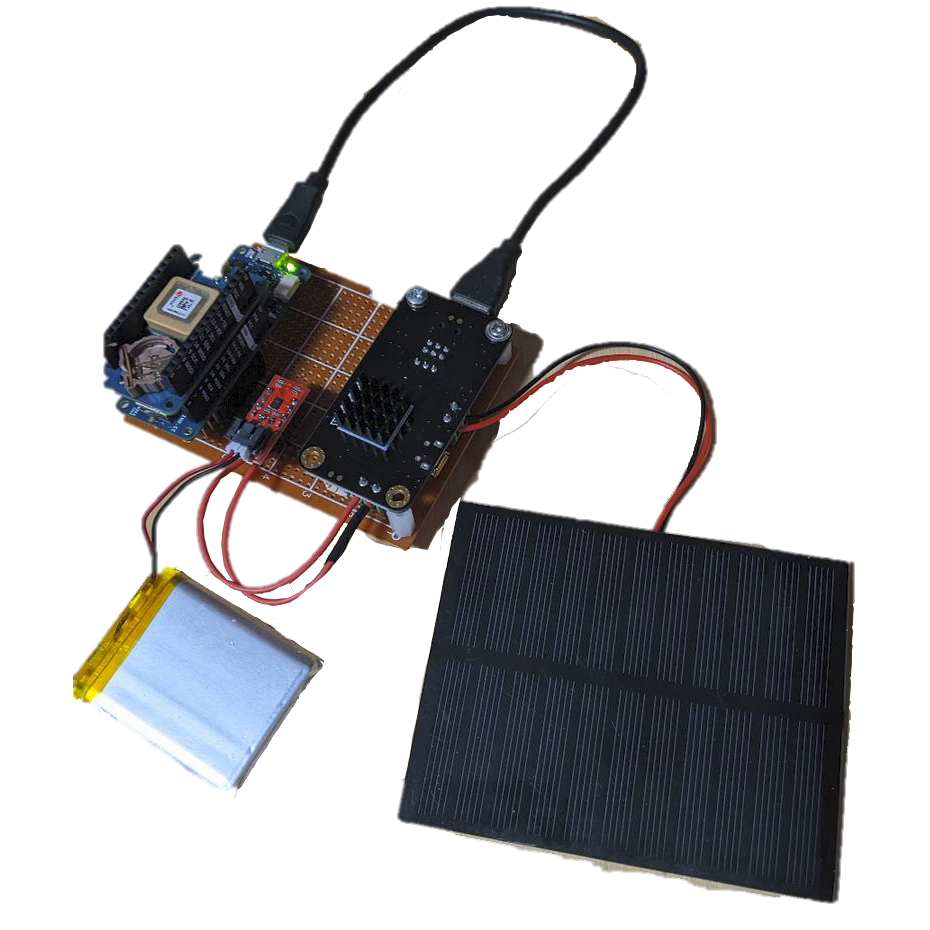
\includegraphics[width=0.5\textwidth]{./figs/prototype_clean.png}
  \caption{Prototype of the reinforcement learning-enabled cattle tracker. The device consists of a solar panel for power harvesting, a rechargeable battery, and an embedded microcontroller for decision-making and communication.}
  \label{fig:prototype}
\end{figure}

The system was evaluated based on its power consumption, data transmission efficiency, and overall performance in real-world conditions. The reinforcement learning algorithm optimized the power usage by balancing data collection, storage, and transmission to ensure continuous operation.

Additionally, the power levels of the device over time were analyzed to assess energy efficiency. Figure~\ref{fig:power_levels} shows the variation in power consumption during different operational phases.

\begin{figure}[htbp]
    \centering
    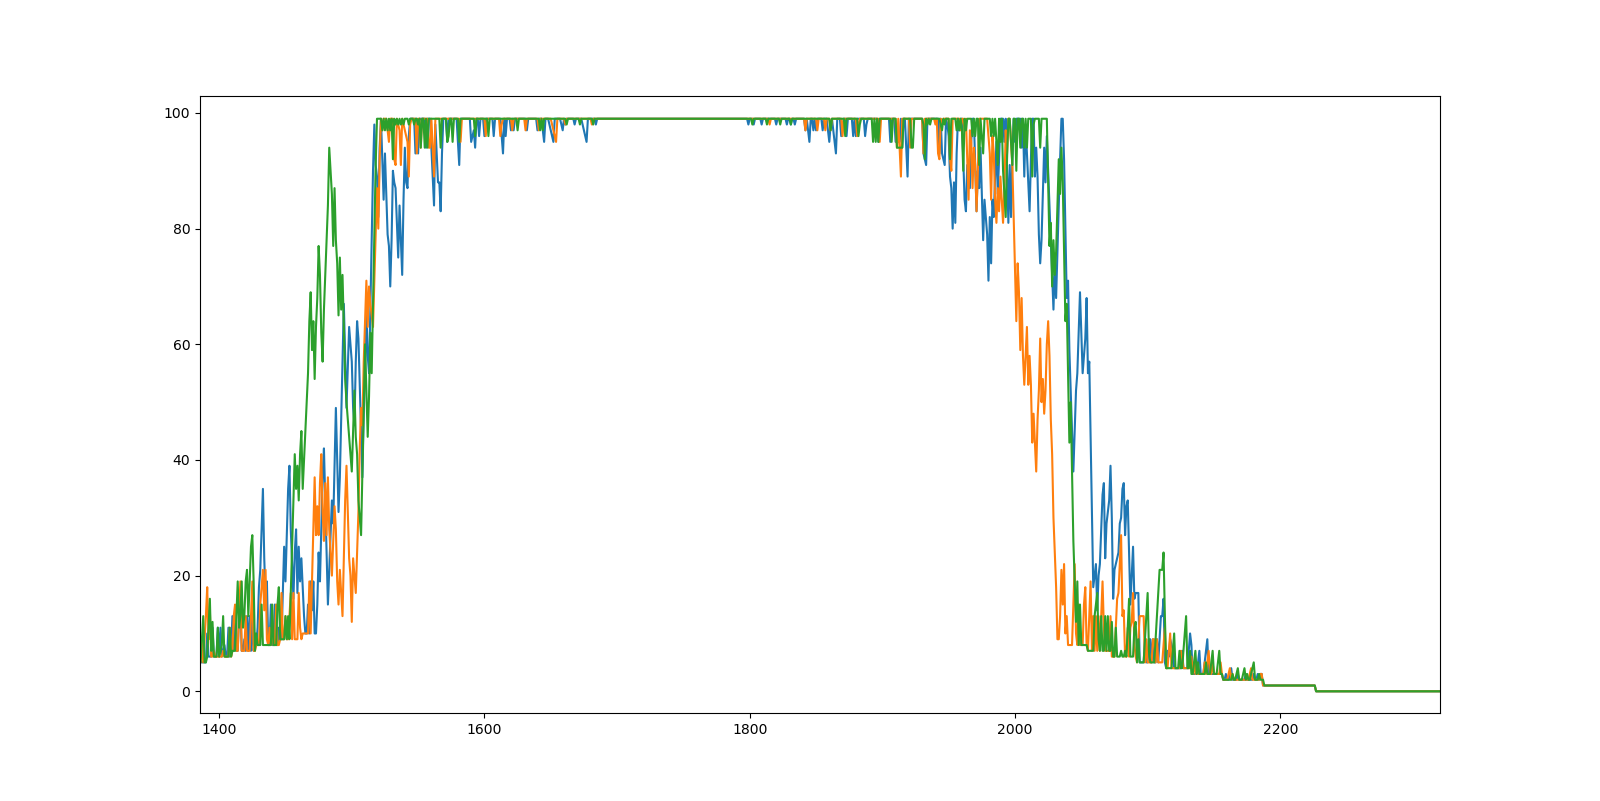
\includegraphics[width=0.8\textwidth]{./figs/power_levels.png}
    \caption{Power consumption levels of the cattle tracker over time. Different colors represent different operational phases such as data transmission, storage, and idle states.}
    \label{fig:power_levels}
\end{figure}

\section{Conclusion}
In this study, we developed a reinforcement learning-enabled cattle tracker prototype designed to optimize power consumption while ensuring efficient data transmission and collection. The device successfully leverages reinforcement learning to dynamically adjust its operation based on available energy, enhancing battery life and operational efficiency. By incorporating solar power and an intelligent decision-making framework, the prototype demonstrates a feasible approach to long-term, autonomous cattle tracking.
Future work will focus on improving the efficiency of the reinforcement learning model by integrating real-time adaptation to environmental changes. Additional experiments in diverse field conditions will provide further validation of the system's robustness. Further refinements to the hardware, such as low-power components and custom PCB design, will enhance reliability and longevity. Moreover, expanding the cloud-based digital twin functionality can improve remote monitoring and predictive analytics for herd management.

\section*{Acknowledgements}

% All references should be stored in the file "references.bib".
% That call to use that file is in "cai.cls". 
% Please do not modify anything below this line.
\printbibliography[heading=subbibintoc]

\end{document}
